\documentclass{sigchi-ext}
% Please be sure that you have the dependencies (i.e., additional
% LaTeX packages) to compile this example.
\usepackage[T1]{fontenc}
\usepackage{textcomp}
\usepackage[scaled=.92]{helvet} % for proper fonts
\usepackage{graphicx} % for EPS use the graphics package instead
\usepackage{balance}  % for useful for balancing the last columns
\usepackage{booktabs} % for pretty table rules
\usepackage{ccicons}  % for Creative Commons citation icons
\usepackage{ragged2e} % for tighter hyphenation
\usepackage{float}
\usepackage{pgfgantt}
\usepackage{pgfgantt-custom}
\usepackage{verbatim}

% \usepackage{marginnote} \usepackage[shortlabels]{enumitem}
% \usepackage{paralist}

%% EXAMPLE BEGIN -- HOW TO OVERRIDE THE DEFAULT COPYRIGHT STRIP --
 \copyrightinfo{Permission to make digital or hard copies of all or
 part of this work for personal or classroom use is granted without
 fee provided that copies are not made or distributed for profit or
 commercial advantage and that copies bear this notice and the full
 citation on the first page. Copyrights for components of this work
 owned by others than ACM must be honored. Abstracting with credit is
 permitted. To copy otherwise, or republish, to post on servers or to
 redistribute to lists, requires prior specific permission and/or a
 fee. Request permissions from permissions@acm.org.\\
 {\emph{CHI'17}}, May 16--May 22, 2017, Copenhagen, Denmark. \\
 Copyright \copyright~2017 ACM ISBN/17/05...\$15.00. \\
 DOI string from ACM form confirmation}
%% EXAMPLE END

\title{GUARDIAN SUIT: Baby monitoring prototype using eTextile to minimize the probability of SIDS}

\numberofauthors{3}
% Notice how author names are alternately typesetted to appear ordered
% in 2-column format; i.e., the first 4 authors on the first column and
% the other 4 authors on the second column. Actually, it's up to you to
% strictly adhere to this author notation.
\author{%
  \alignauthor{%
    \textbf{Madrigal N. Totayo}\\
    \affaddr{University of Copenhagen} \\
    \affaddr{Universitetsparken 5} \\
    \affaddr{2100 Copenhagen} \\
    \affaddr{vnw888@alumni.ku.dk} } \vfil \alignauthor{%
    \textbf{Mark Wulff}\\
    \affaddr{University of Copenhagen}\\
    \affaddr{Universitetsparken 5}\\
    \affaddr{2100 Copenhagen} \\
    \email{lrh211@alumni.ku.dk} }  \vfil \alignauthor{%
    \textbf{Mark J. Jacobi}\\
    \affaddr{University of Copenhagen}\\
    \affaddr{Universitetsparken 5}\\
    \affaddr{2100 Copenhagen} \\
    \email{dcz738@alumni.ku.dk} } }

% Paper metadata (use plain text, for PDF inclusion and later
% re-using, if desired)
\def\plaintitle{SIGCHI Extended Abstracts Sample File: Note Initial
  Caps} \def\plainauthor{First Author, Second Author, Third Author,
  Fourth Author, Fifth Author, Sixth Author}
\def\plainkeywords{SIDS; eTextile; monitoring; breathing; lying position.}
\def\plaingeneralterms{Documentation, Standardization}

%% Set up our PDF with metadata
\hypersetup{%
  pdftitle={\plaintitle}, pdfauthor={\plainauthor},
  pdfkeywords={\plainkeywords}, }

% \reversemarginpar%

\begin{document}

\maketitle

% Uncomment to disable hyphenation (not recommended)
% https://twitter.com/anjirokhan/status/546046683331973120
\RaggedRight{} 

% Do not change the page size or page settings.
\begin{abstract}
  The most important rule of Abstracts is that they describe the work, not the paper. Include, at most, one sentence of motivation. Save the rest of your motivation for the Introduction. Effective Abstracts focus on two things: (1) Describing what was done. (2) Describing what was found (key results). Be specific about your key findings. Instead of "many" say "84\%". Keep the Abstract to one paragraph and fewer than 200 words.
\end{abstract}

\keywords{\plainkeywords}

\category{J.3}{Health and Medical systems}{Medical information systems}
% See http://www.acm.org/about/class/ccs98-html for all (men denne er den eneste som passer til os)

\section{Introduction}
Since the early 1960s and 1970s \cite{aap-1992} infants have been victims for Sudden Infant Death Syndrome (SIDS)\footnote{\url{https://en.wikipedia.org/wiki/Sudden_infant_death_syndrome}}, which is the case where the infants are found dead in their last place of sleep. Since then, many recommendations for the infants sleeping positions and environments has been made in order to lower the probability of SIDS which unfortunately still occurs. After many years of research from 1992-2004 by the American Academy of Pediatrics (AAP) \cite{aap-1992,aap-1996,aap-2005} the main recommendations for minimizing the probability of SIDS is to detect:
\begin{itemize}
  \item Whether the infant is breathing or not.
  \item When the infant changes position.
\end{itemize}
Many products have been developed, with the purpose of monitoring the baby (e.g. critical shifts in the temperature of the room). A majority of these products have an object present near the infant's crib, which we find to be rather clunky and can be misleading (i.e. false positives). Instead, in this paper we propose a onesie with eTextiles embedded into it. These eTextiles has the capability of increasing the resistance when stretched and when applying pressure. We developed Guardian Suit, a onesie with one-dimensional textile sensors sewn into it as such: (1) around the chest area, (2) on the lower-back, (3) stomach, and (4) one on each side.

The first sensor introduced is a piezoresistive elastic polymer that can increase the resistance when stretched. This allows for detecting whether the infant is breathing or not. The sensors for the sides, stomach and back are made by putting a piece of piezoresistive fabric in-between two pieces of conductive fabrics. They decrease in resistance when pressure is applied to them. These sensors are placed as such in order to detect whether the infant is in a prone (i.e. on the stomach), supine (i.e. on the back) or lateral (i.e. on the side) position.

Furthermore, as our product is electrical, we don't want the possibility of hurting the baby e.g. by getting electrocuted. For this, we created strips out of conductive fabric that were sewn into the onesie. These are then connected to the development board by crimping the sensors\footnote{\url{https://www.pololu.com/product/1928\#lightbox-picture0J3280;main-pictures}} or by using snaps\footnote{\url{https://www.sparkfun.com/products/11347}}.

\colorbox{cyan}{Something about key results of what we did. Major findings}.

In the following, we will describe our findings of how the infant should interact with the artifact. Thus, we had to build it with the following in mind:
\begin{itemize}
  \item Sensor construction and placement techniques.
  \item Connecting the sensors to the development board without the use of wires.
  \item Usage scenarios and possible feedback from the readings.
\end{itemize}

\section{Related work}
As mentioned earlier, many products has been developed with the intention of preventing SIDS. One of them is the Georgia Tech Wearable Motherboard (GTWM)\footnote{\url{http://www.gtwm.gatech.edu/}}. Initially developed in collaboration with the US Navy Department to monitor a soldier's vital signs by detecting the penetration of e.g. bullets and shrapnel, it was later augmented to monitor an infant's breathing or heart rate by using cardiorespiratory sensors on a vinyl strap, as described by Fantauzzacoffin et al. \cite{p285-fantauzzacoffin}. The engineers had created it by weaving signal transmission lines and integrated the sensors into a onesie. Even though one mother didn't mind her infant to be surrounded by wires from the device, and found it to be quite comfortable, there might be a possibility that the statement was biased as no other test subjects has been mentioned or found.

Kroutil et al. \cite{a33-kroutil} used electrically conductive stranded yarn as sensors, placed underneath the lower bed sheet to detect respiration among individuals. 

%\begin{comment}
\marginpar{%
  \vspace{-45pt} \fbox{%
    \begin{minipage}{0.925\marginparwidth}
    \textbf{Creating the breathing sensor} \\
      \begin{figure} [H]
    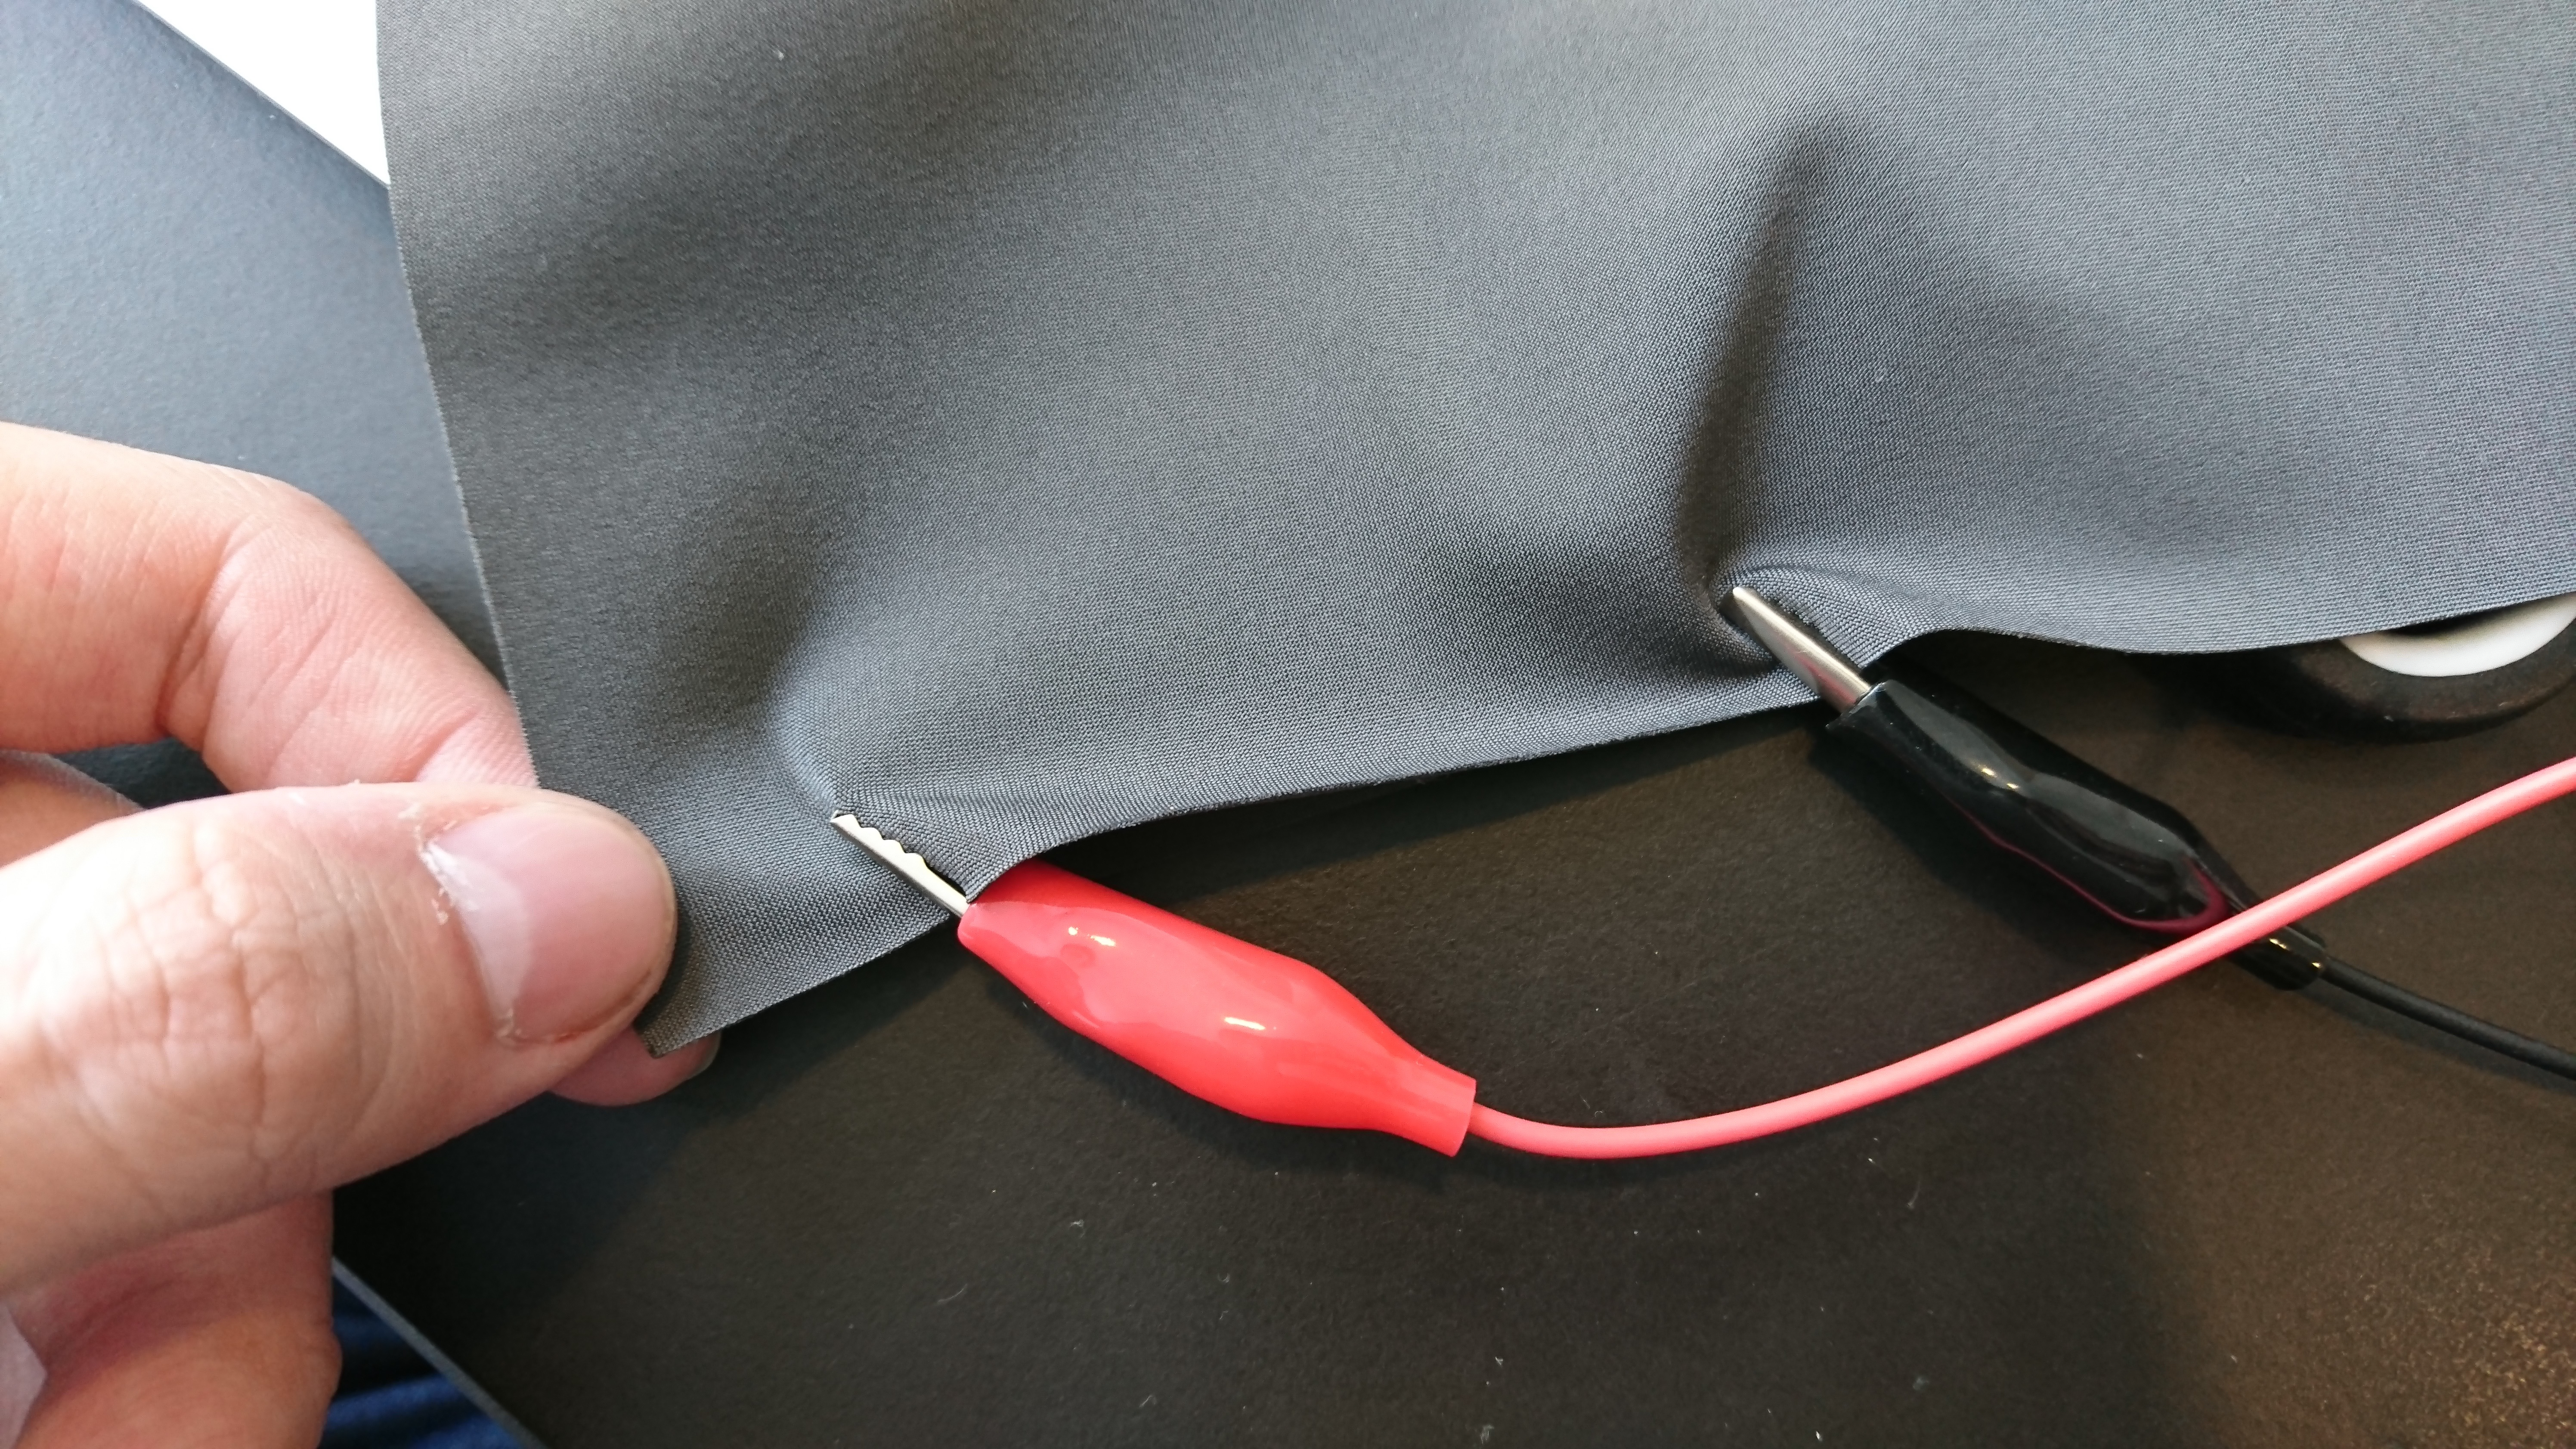
\includegraphics[width=1.0\textwidth]{img/breathing_sensor}
    \caption{Test of the piezoresistive elastic polymer using crocodile clip wires.}
\end{figure}
\begin{figure} [H]
    \includegraphics[width=1.0\textwidth]{img/sewing1}
    \caption{Sewing.}
\end{figure}
\begin{figure} [H]
    \subfigure\includegraphics[width=1.0\textwidth]{img/sewing2}
    \subfigure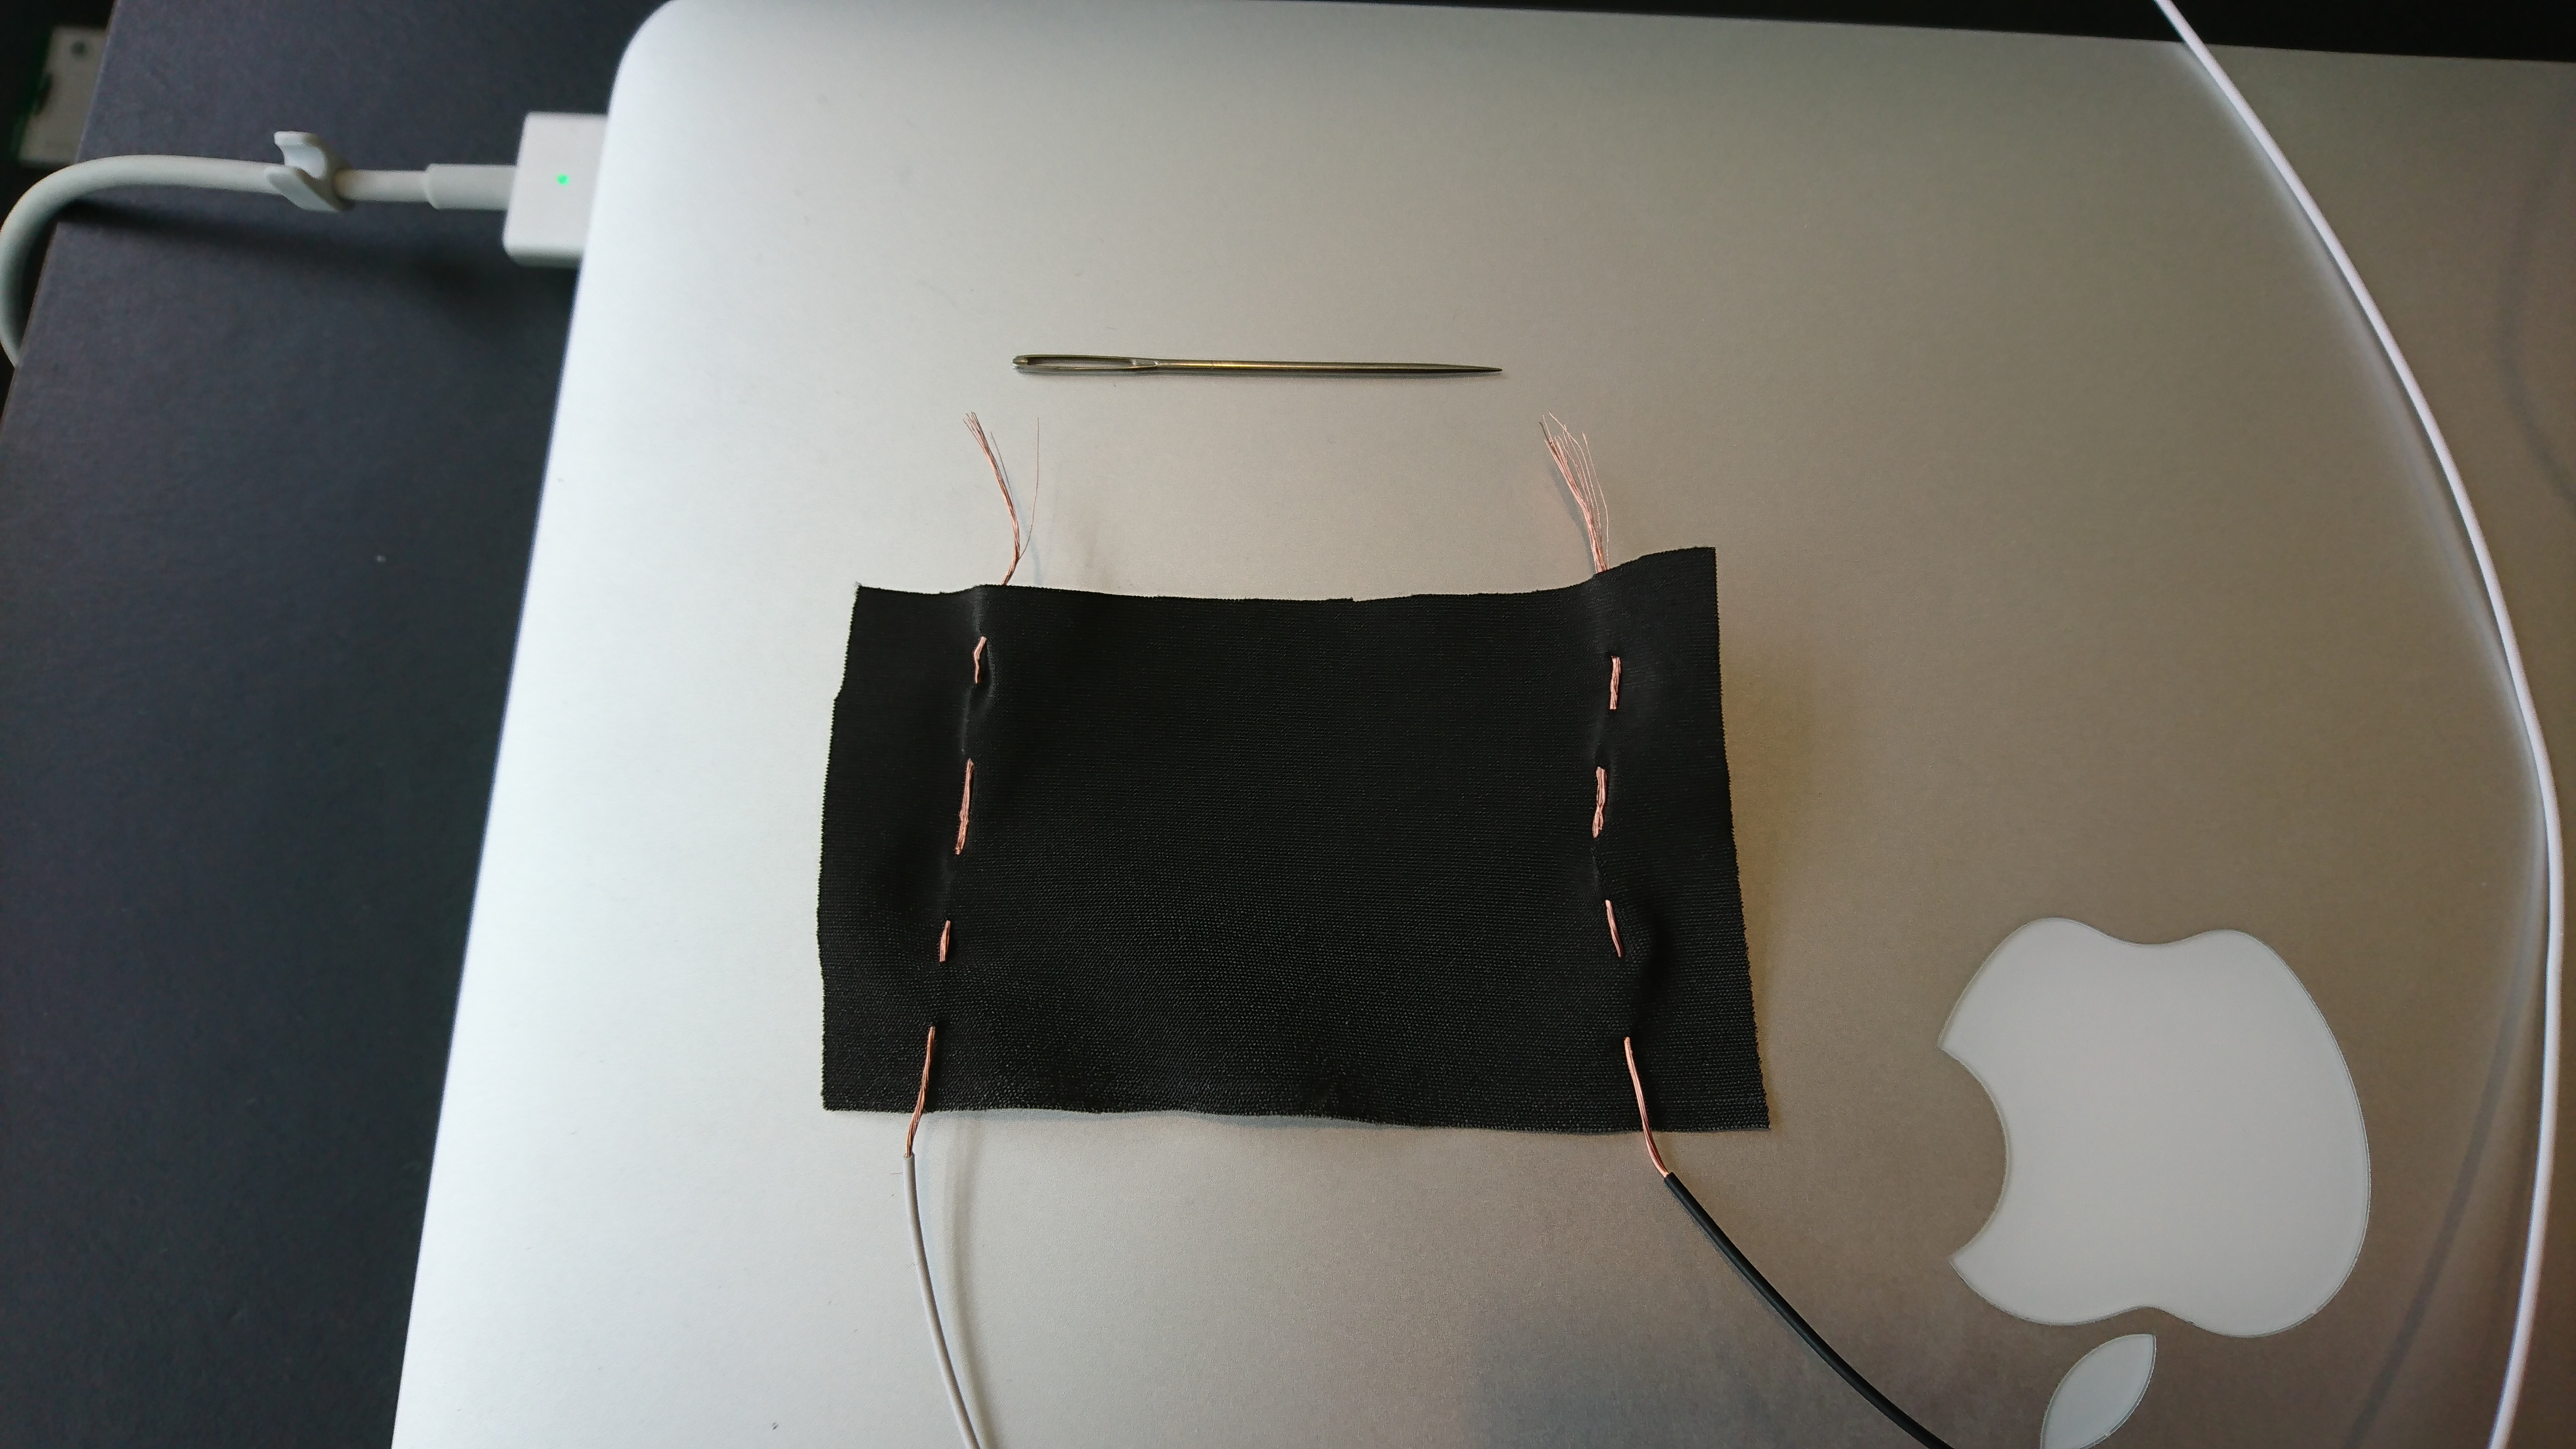
\includegraphics[width=1.0\textwidth]{img/sewing3}
    \caption{A bit more sewing.}
\end{figure}
    \end{minipage}}\label{sec:sidebar} }
%\end{comment}

    The sensors measured the respiratory activity by the alteration of electrical capacitance of the chest area. This was done so one could monitor patients respiration without inconveniencing them with wiring and sensors attached to their bodies.

Another bedsheet monitor was proposed by Huang et al. \cite{a18-huang}. Embedded with pressure sensors and in conjunction with collated data, they were able to detect whether the person was breathing or not within a certain time interval, corresponding to a predetermined minimum breathing rate.

Even though creating the sensors within the fabric of the surface the infant is lying on during sleep has produced satisfactory results \cite{a18-huang, a33-kroutil}, we have chosen another approach. Guardian Suit combines the wearability, comfort, and ease of use of GTWM\footnote{\url{http://www.gtwm.gatech.edu/}} \cite{p285-fantauzzacoffin} with the pressure sensing technologies used in the bedding solutions. We receive feedback whenever the infant is in either position i.e. prone (stomach), supine (back) or lateral (side). With the electrical elastic polymer described earlier we are able to detect the breathing rate of the baby. Finally, with constraints as proposed by Huang et al. \cite{a18-huang}, we can detect whenever any individual is in a critical state.

We will try to utilize piezoresistive conductive
stretchable fabric. However, as a fallback, the 
research of Vogl et al.\cite{stretcheband}
tests various stitching patterns and the resistance measured
when stretching the stitching some amount. This could 
potentially benefit us for the breathing sensor if the piezoresistive conductive
stretchable fabric proves insufficient.

%\colorbox{cyan}{+ something about eTextiles in general perhaps}.

\section{Artifact construction}
All of the materials used are relatively cheap, but depending on one's location,
it may be difficult to obtain. Our location, i.e. Denmark, required shipping of
the eTextile material from the USA.
Material needed and convenient tools or other materials can be seen below.
\begin{figure} [H]
  \centering
    \includegraphics[width=0.35\textwidth]{img/materials}
    \caption{An overview of all our materials.}
\end{figure}
Of the necessary materials to produce the sensors, we need the following:
\begin{itemize}
  \item Piezoresistive fabric.
  \item Piezoresistive elastic polymer.
  \item Conductive fabric.
  \item Sewing equipment or similar (to combine the fabrics).
  \item Wires (for connecting the arduino to the breadbord).
  \item Micro-controller.
\end{itemize}

And for our prototype and convenient materials:
\begin{itemize}
  \item Baby-sized onesie.
  \item Non-conductive regular fabric.
  \item Crocodile clip wires.
  \item Wire stripper.
\end{itemize}

%\begin{comment}
\marginpar{%
  \vspace{-65pt} \fbox{%
    \begin{minipage}{0.925\marginparwidth}
      \begin{figure} [H]
   \centering \includegraphics[width=0.85\textwidth]{img/chest}
    \caption{The stretching part for the artifact.}
\end{figure}
\begin{figure} [H]
    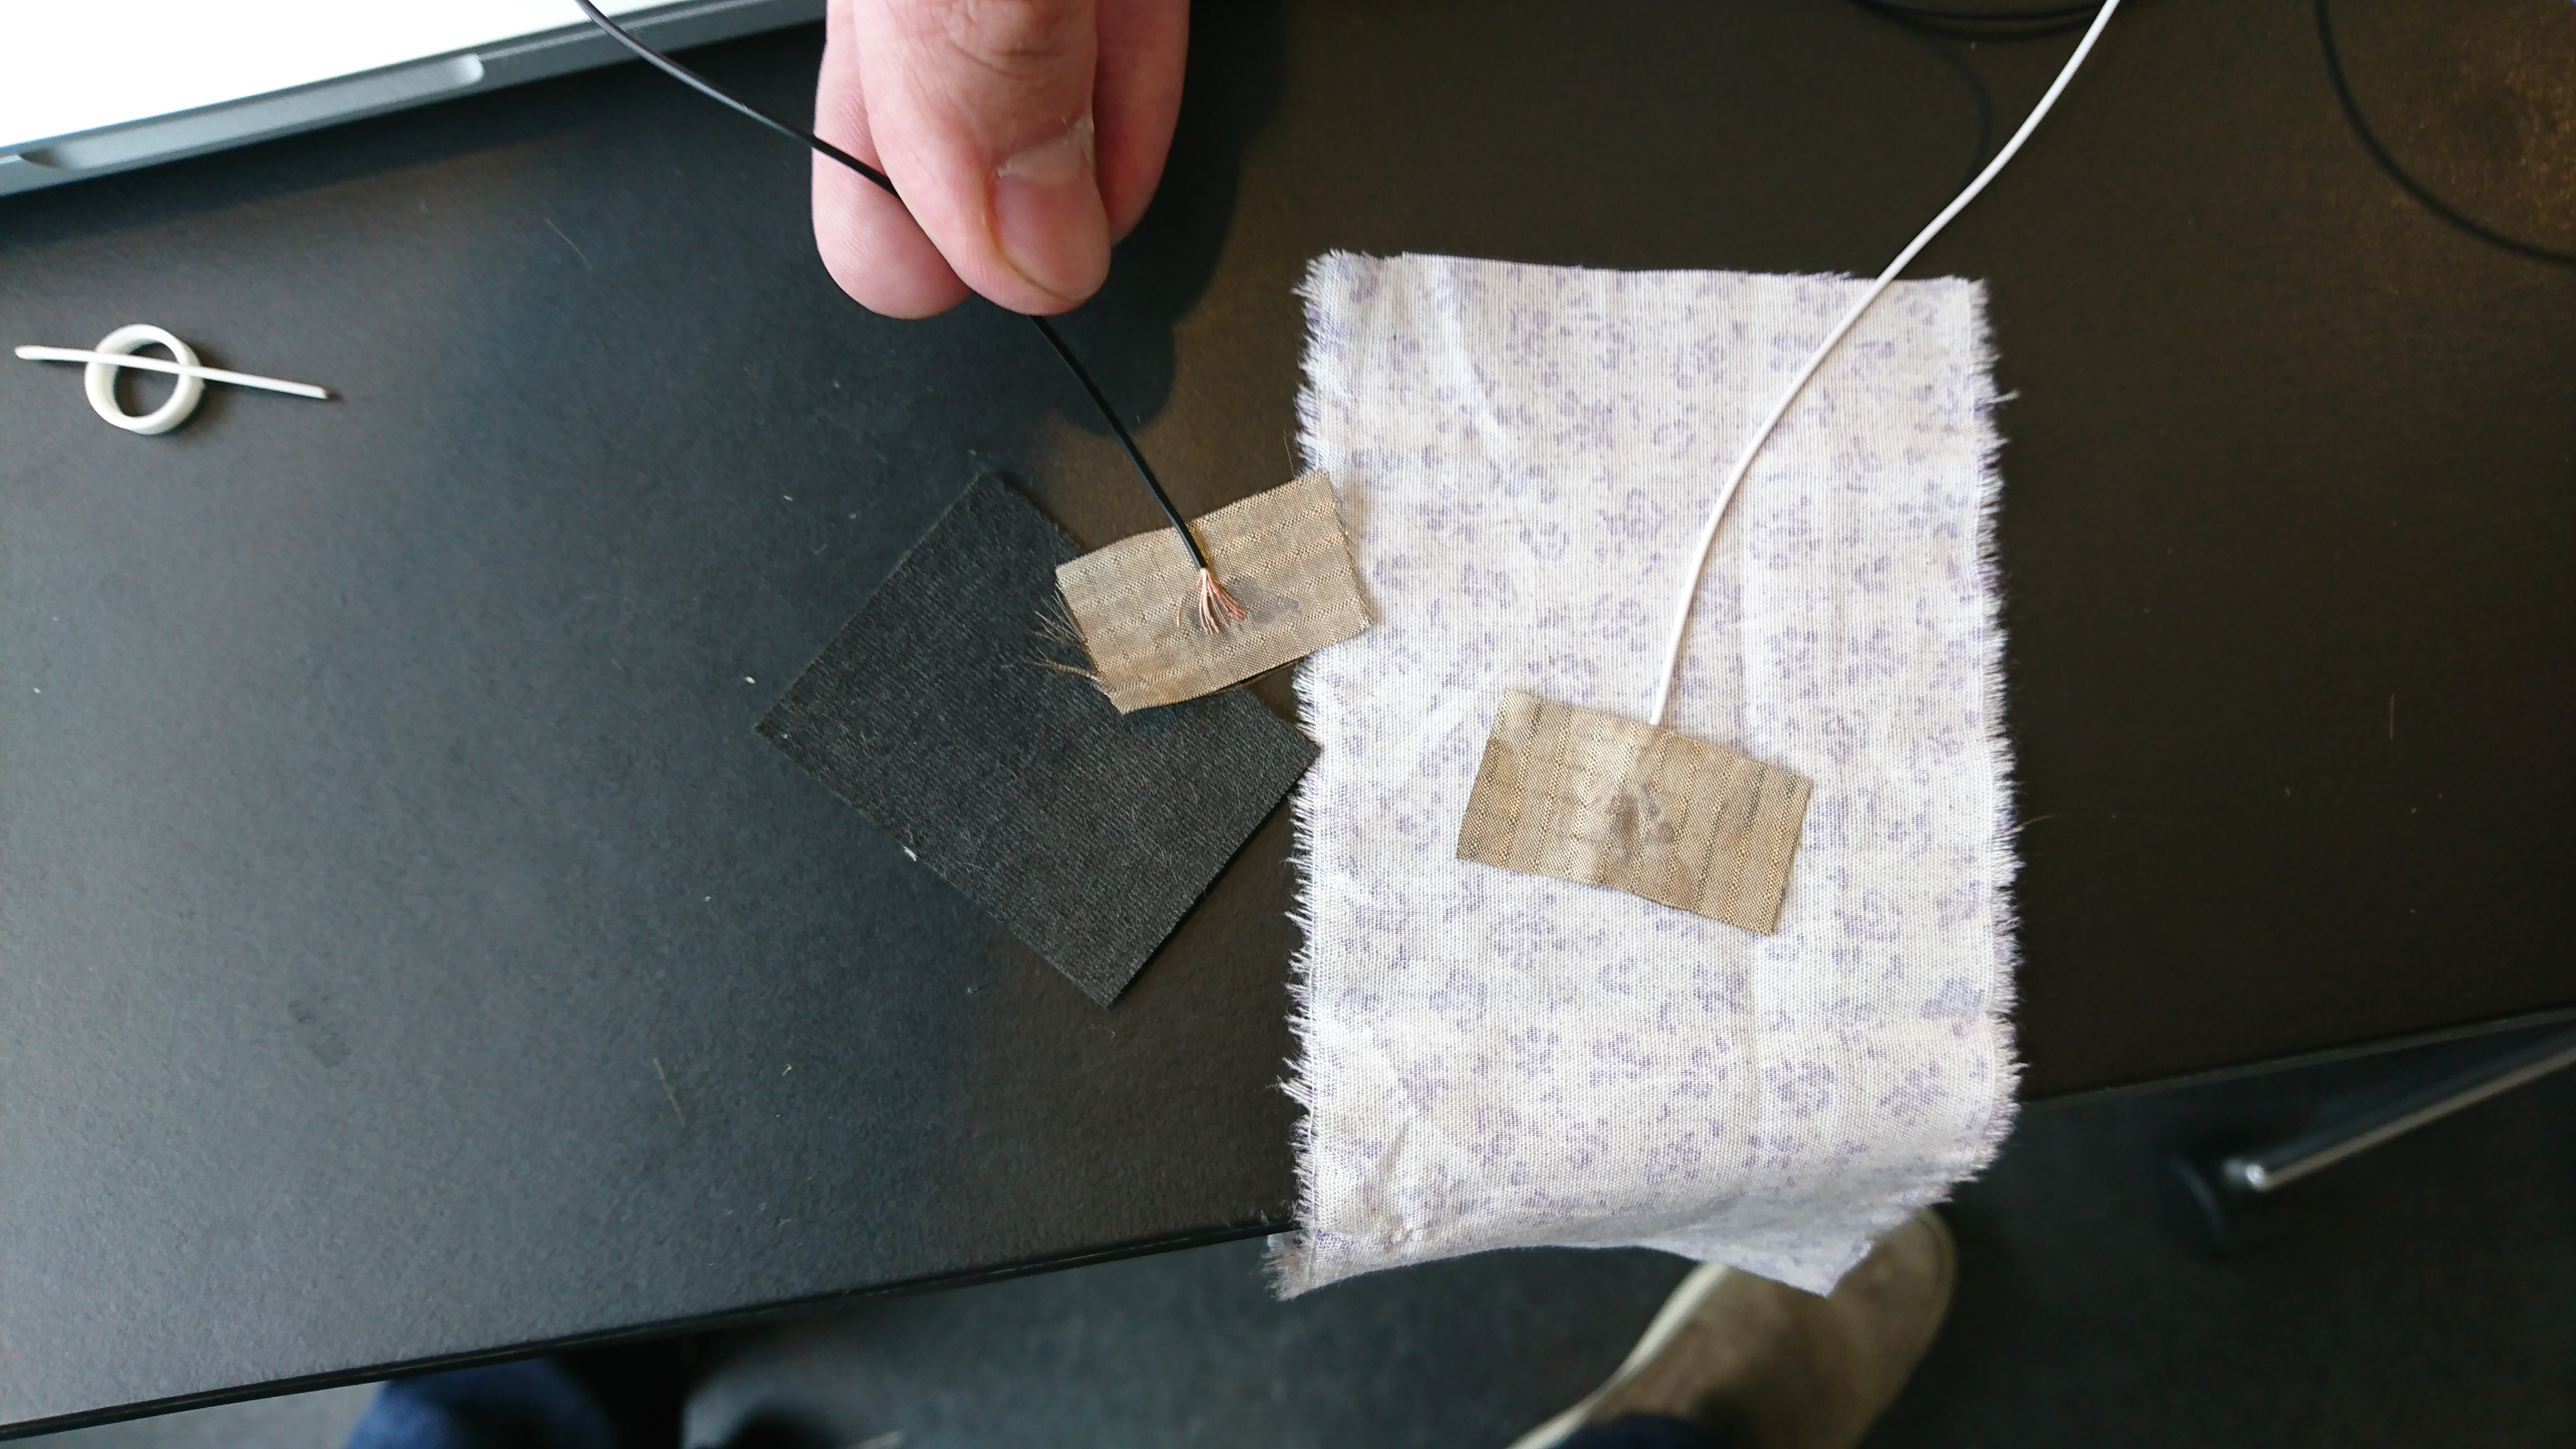
\includegraphics[width=1.0\textwidth]{img/pressure_sensor}
    \caption{The two conductive fabrics (gold), the piezoresistive fabric (black)
and the non-conductive wrapping fabric (white). 1.4 mm wires attached with a
touch of super glue (non-conductive) to keep them on the fabric.}
\end{figure}
\begin{figure} [H]
    \includegraphics[width=1.0\textwidth]{img/pressure_pad}
    \caption{Pressure pad (held together with needles).}
\end{figure}
    \end{minipage}}\label{sec:sidebar2} }
%\end{comment}

\subsection{Breathing sensor}
For the breathing sensor we will use the EeonTex piezoresistive elastic polymer.
This polymer has the property that the resistance is increased when the fabric
is stretched.
Before constructing the prototype, we tested the polymer by simply putting
crocodile wires on two ends of a piece, and then stretching it by hand.

After verifying that the resistance increases by a simple Arduino-program which
measures the pull-up resistance, we took some wire and stripped a large section
of the end, and sewed this into the ends of the elastic polymer.

To test the breathing sensor, we applied the pad to ourselves by attaching the pad to a
non-elastic fabric slip which can be fitted around the chest of an adult.

After trying the sensor on an adult we experienced sensor readings fluctuating
with 100 points in resistance with heavy breathing and 30 with regular breathing.

From the initial strip of material we had access to, the 
amount of resistance we were able to measure were 
insufficient to properly determine breaths. We also tested
the sensor in a lying down position and can assume
that the user will lie somewhat still during sleep. The
sensor would actuate more easily when flexing muscles. 
From the consultation of some eTextile experts, three 
suggestions to make the sensor more sensitive will
be tested.

\begin{itemize}
  \item A long thin strip of the piezoresistive elastic
  stretch fabric.
  \item A coiled piece of the piezoresistive elastic
  stretch fabric (can be made from the long thin strip in
  the previous suggestion).
  \item Various lengths and widths of the the piezoresistive
  elastic stretch fabric.
\end{itemize}

To test the three different material sizes, we did this in accordance to the amount the chest changes in circumference. We measured the circumference of the chest when fully
exhaled, fully inhaled and a regular breath (this will vary depending on person).

\begin{table}
  \centering
  \begin{tabular}{l r}
    % \toprule
    & \multicolumn{1}{l}{\small{\textbf{Breath circumference measure}}} \\
    \cmidrule(r){1-2}
    {\small\textit{State}}
    & {\small \textit{circumference (cm)}} \\
    \midrule
    Full exhale    & 101.0 \\
    Full inhale    & 107.0 \\
    Regular exhale & 104.2 \\
    Regular inhale & 105.5  \\
    % \bottomrule
  \end{tabular}
  \caption{Measurements of chest circumference when breathing. Used for testing the Eeontex material.}~\label{tab:circumference}
\end{table}

From the above table we get an idea of how much a single breath affects the circumference
in an adult male. Though this is not representative of a baby, due to the 
inaccessibility of one and that we want to develop a first iteration prototype, this
will be our basis of the breath sensor.\\
We see that the difference in a full forced inhale/exhale is around 6 cm. whereas regular
breathing only results in around 1 cm in difference.\\
We have experimented with the different sizes of the Eeontex conductive piezoresistive 
stretch fabric. From the breath circumference table we can see the change varies in cm and
now constructs a simple experiment in order to evaluate the change in resistance given 
different fabric sizes.\\
%\begin{comment}
\marginpar{%
  \vspace{-95pt} \fbox{%
    \begin{minipage}{0.925\marginparwidth}
      \begin{figure} [H]
   \centering 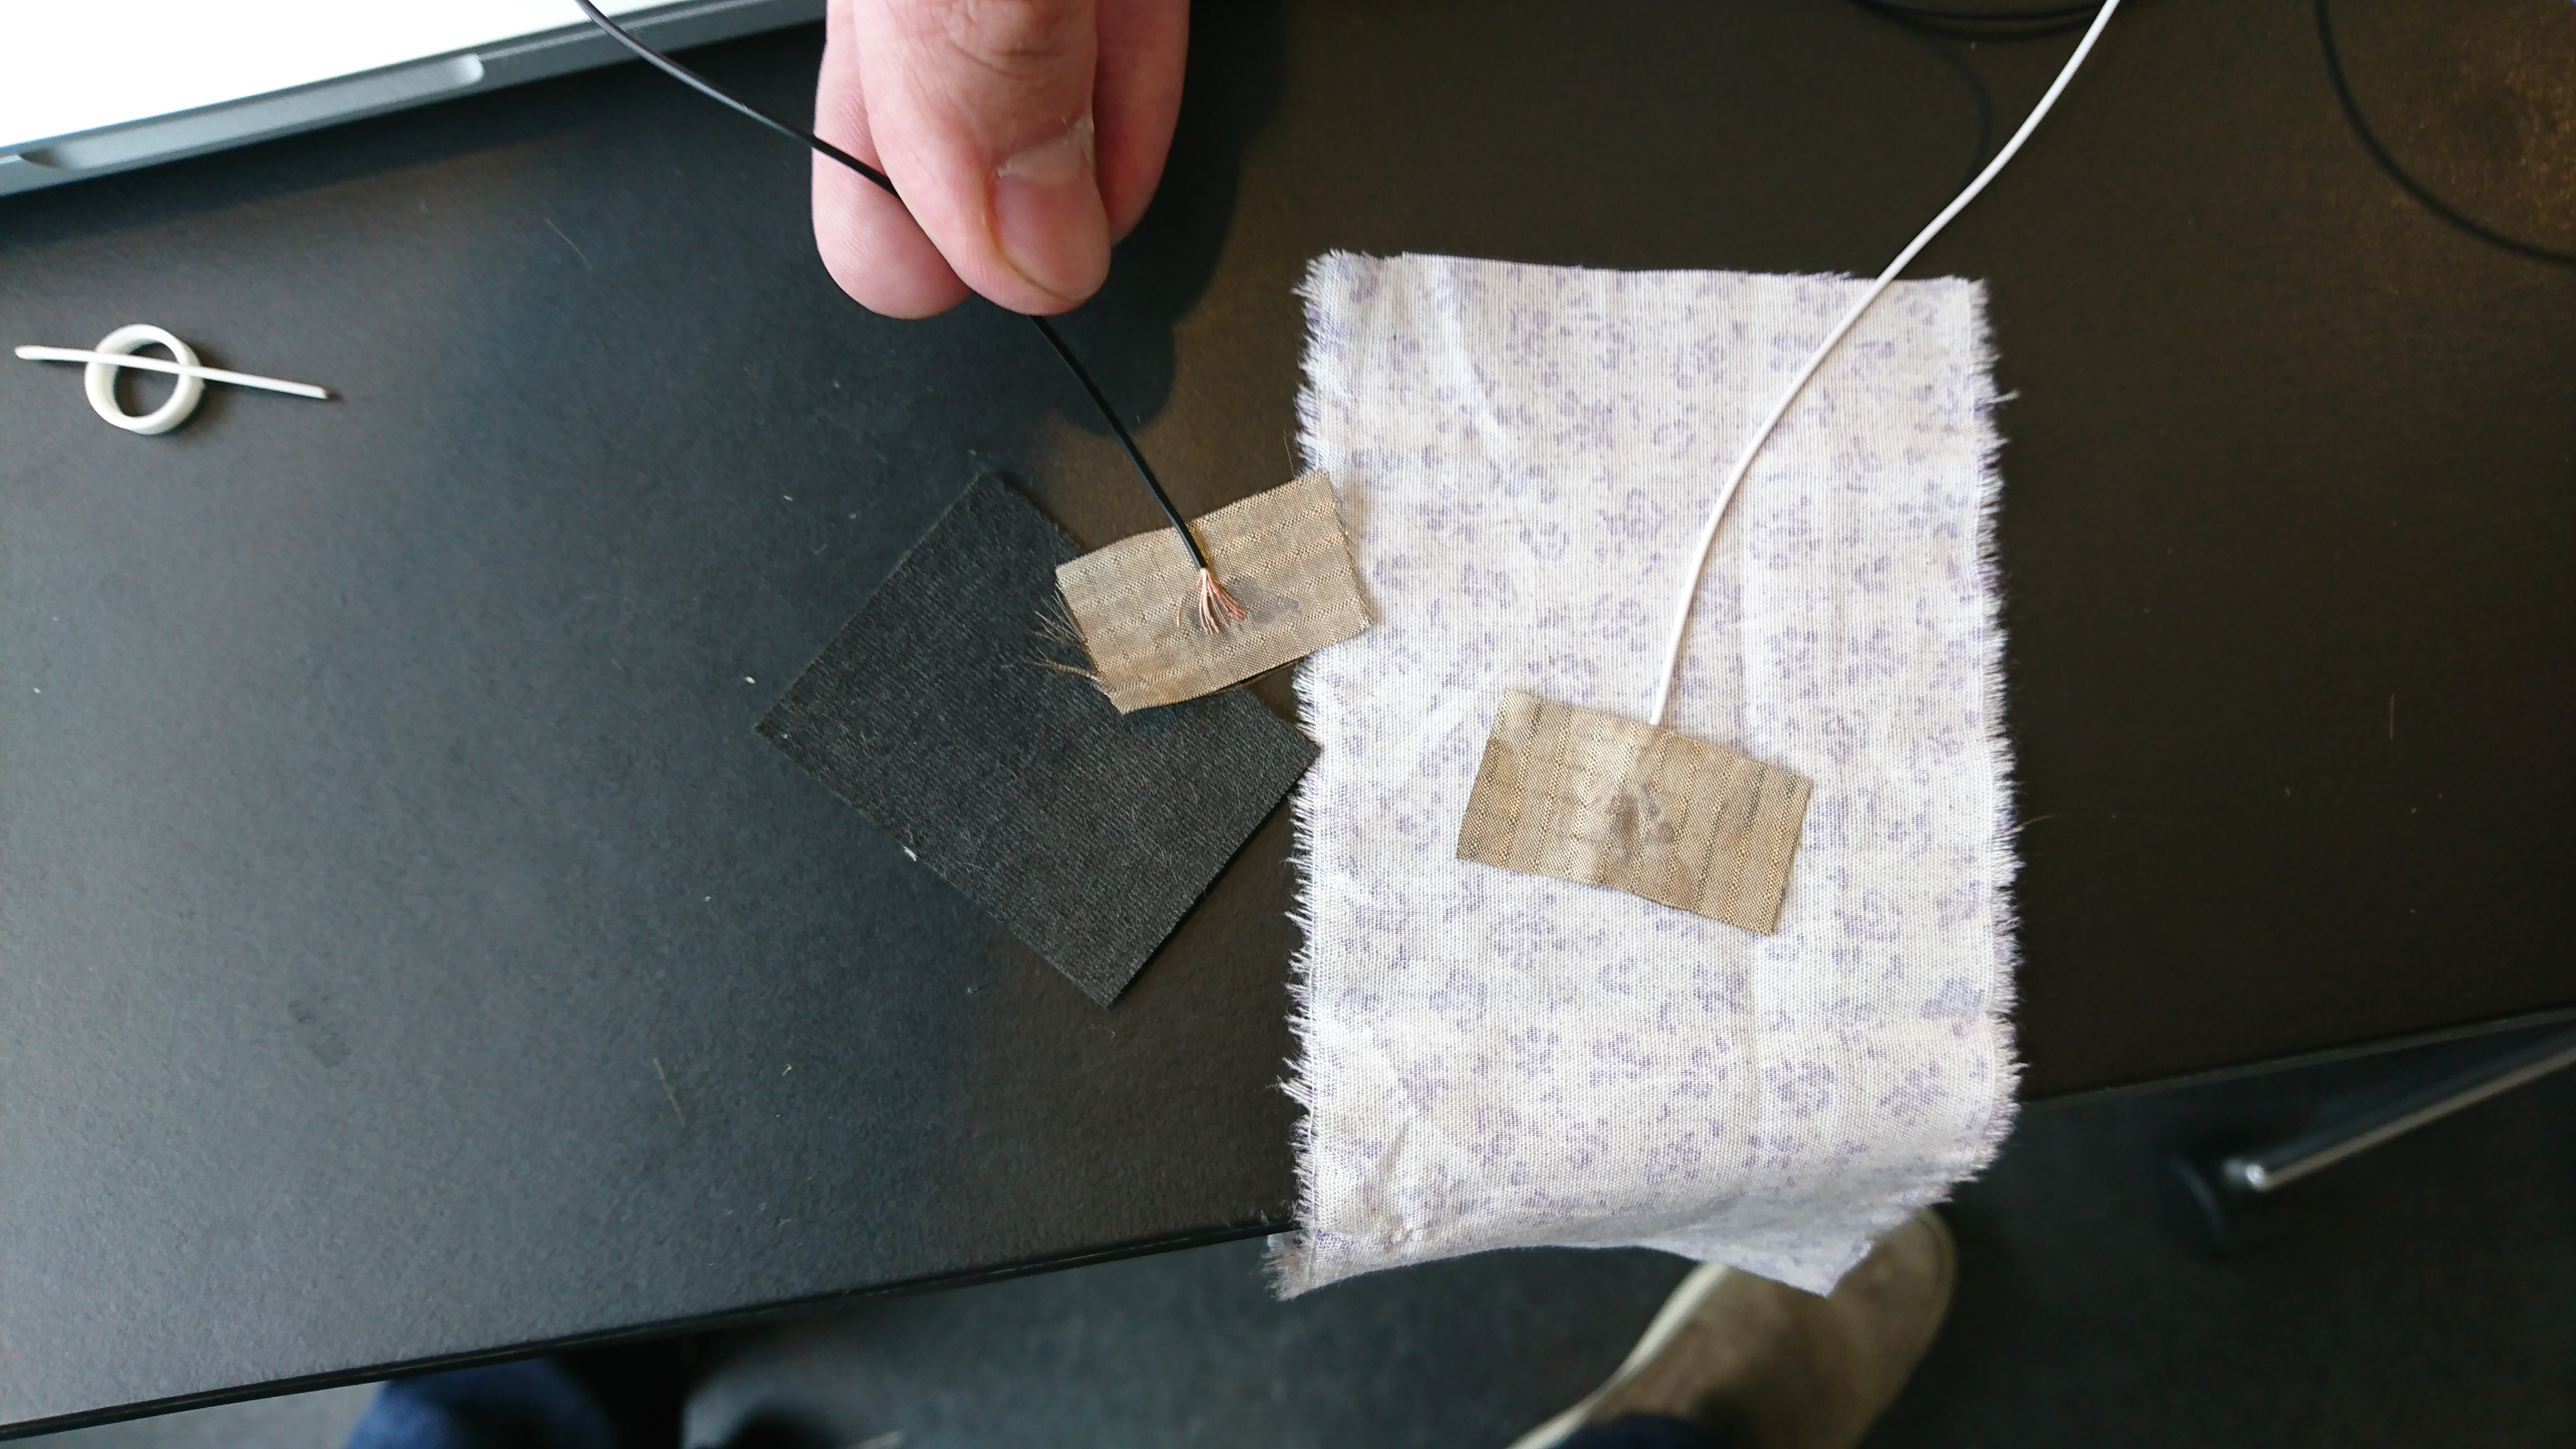
\includegraphics[width=0.85\textwidth]{img/pressure_sensor.jpg}
    \caption{The prototyping of the eTextile pad.}
\end{figure}
      \begin{figure} [H]
   \centering 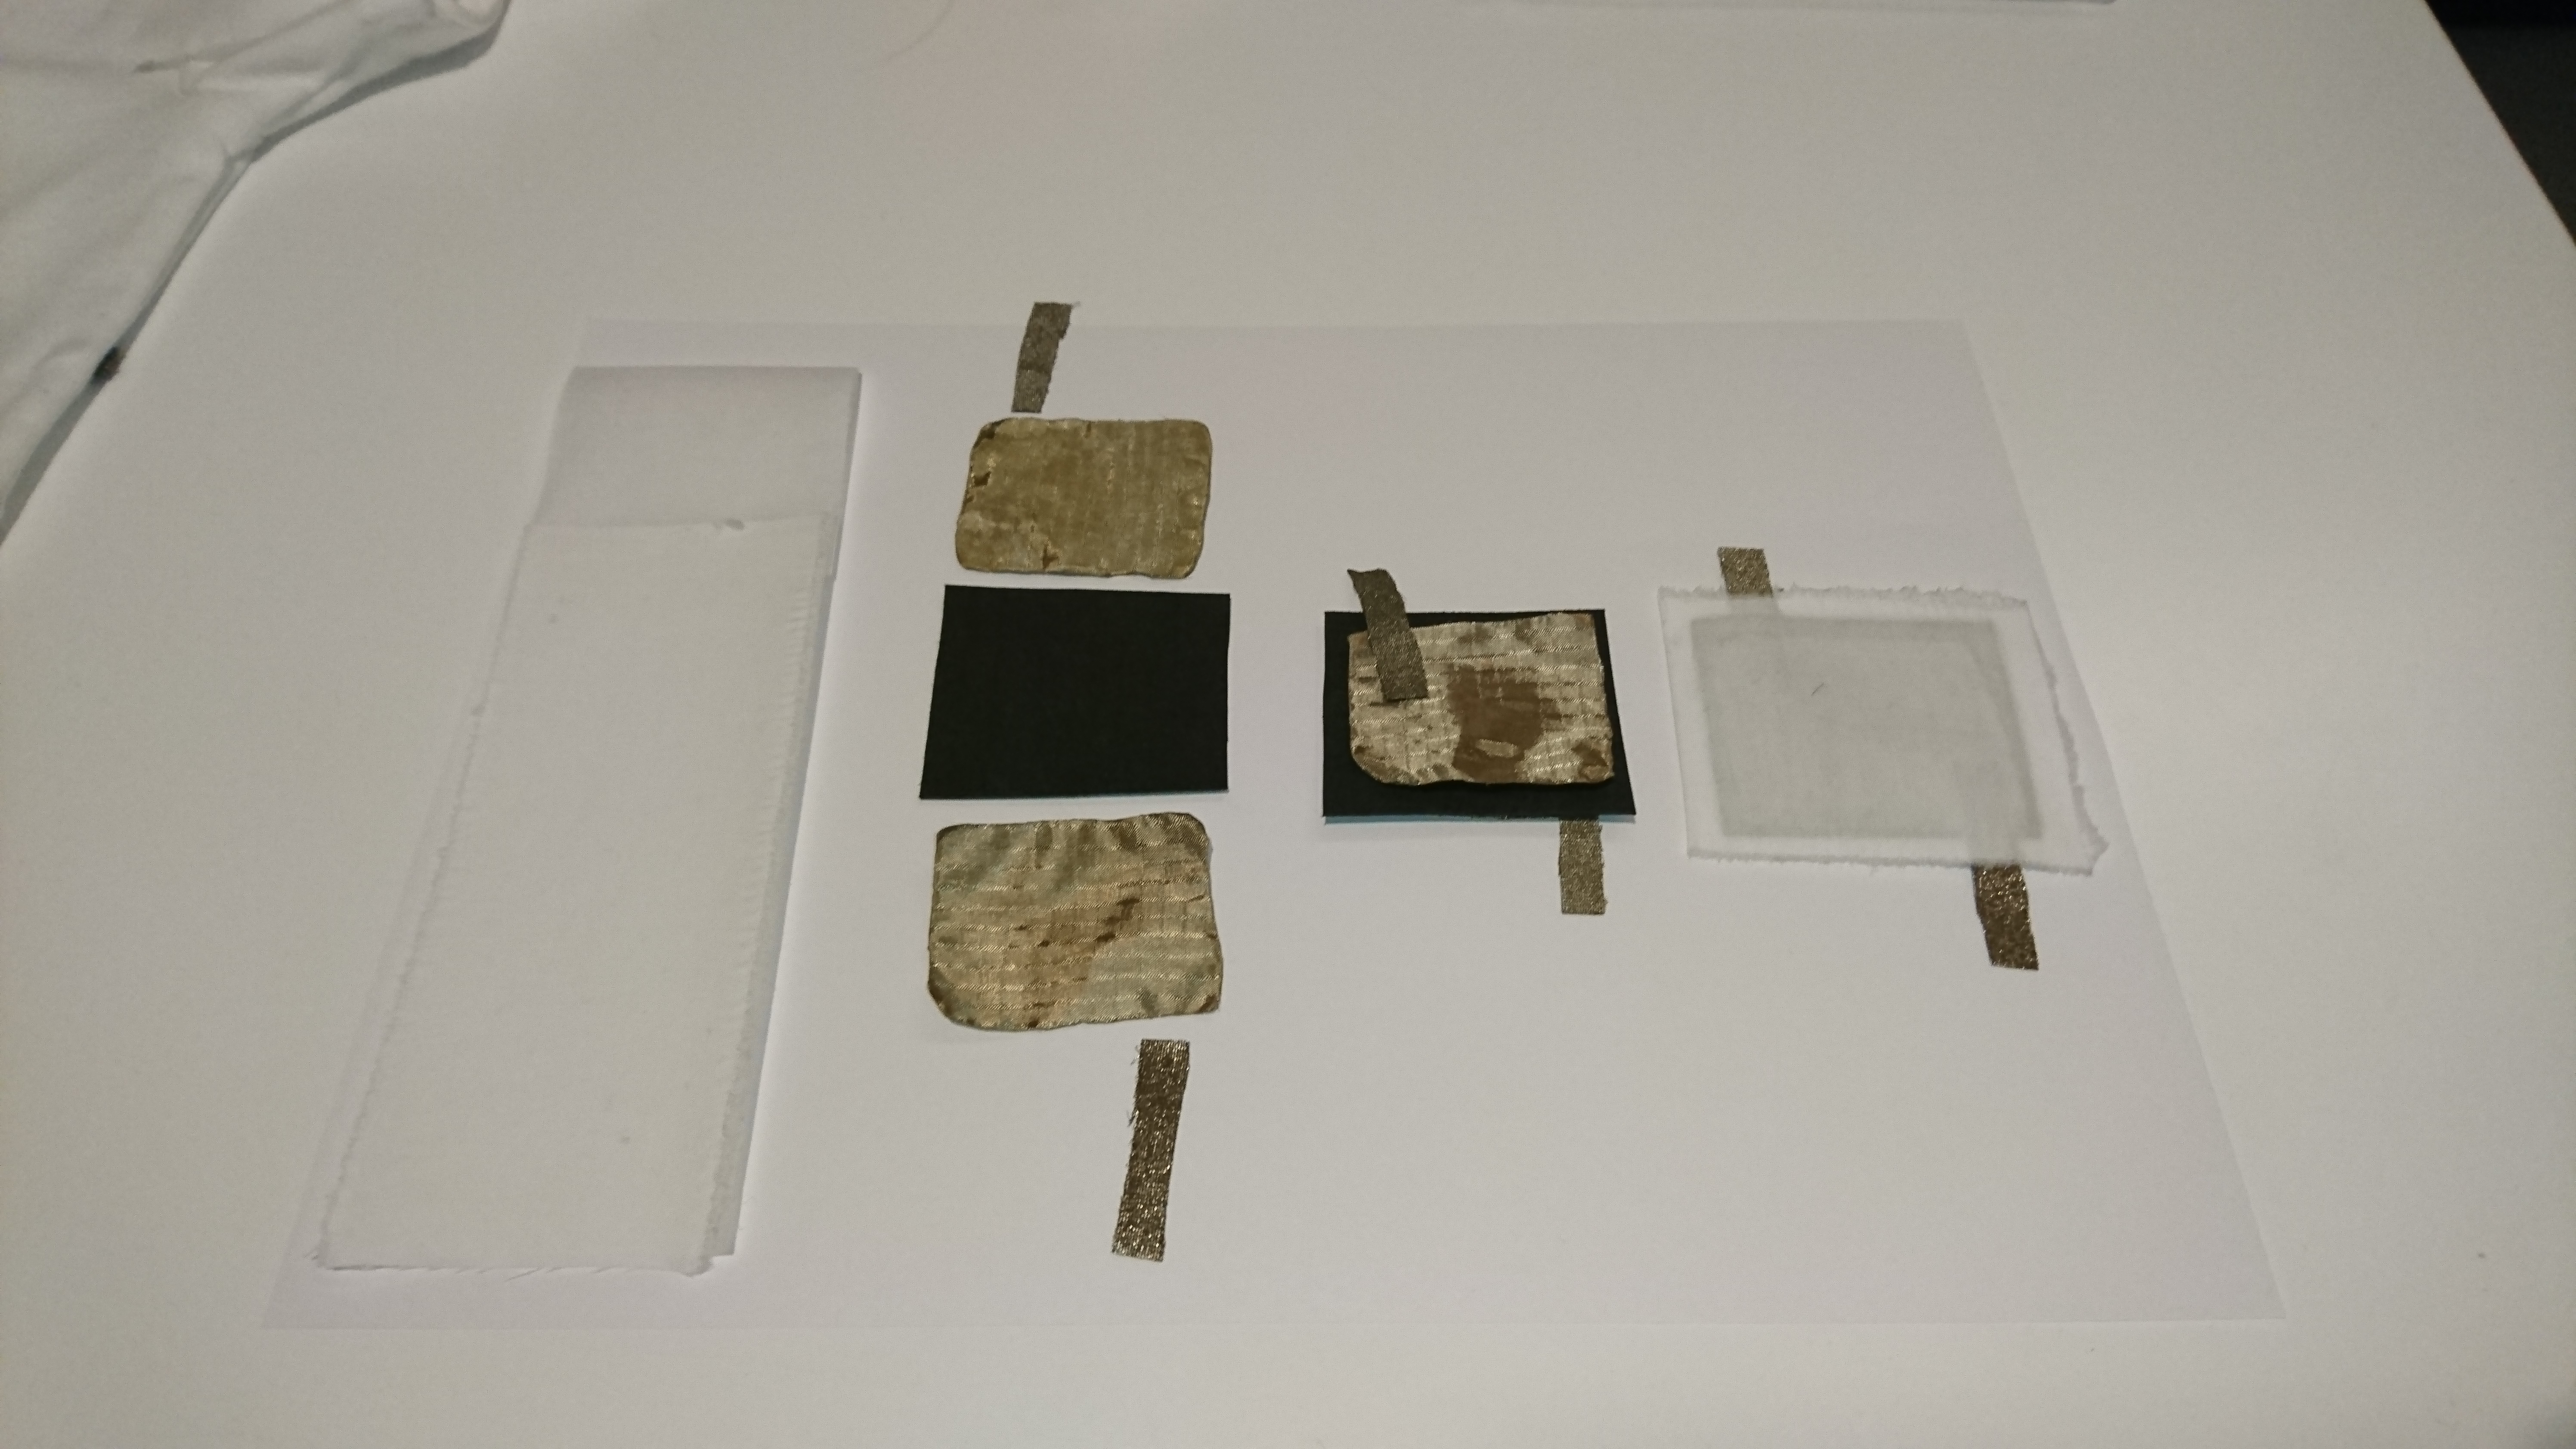
\includegraphics[width=0.85\textwidth]{img/pressure_sensor2.JPG}
    \caption{Overview of the final pressure sensor construction (materials and assembly).}
\end{figure}
      \begin{figure} [H]
   \centering 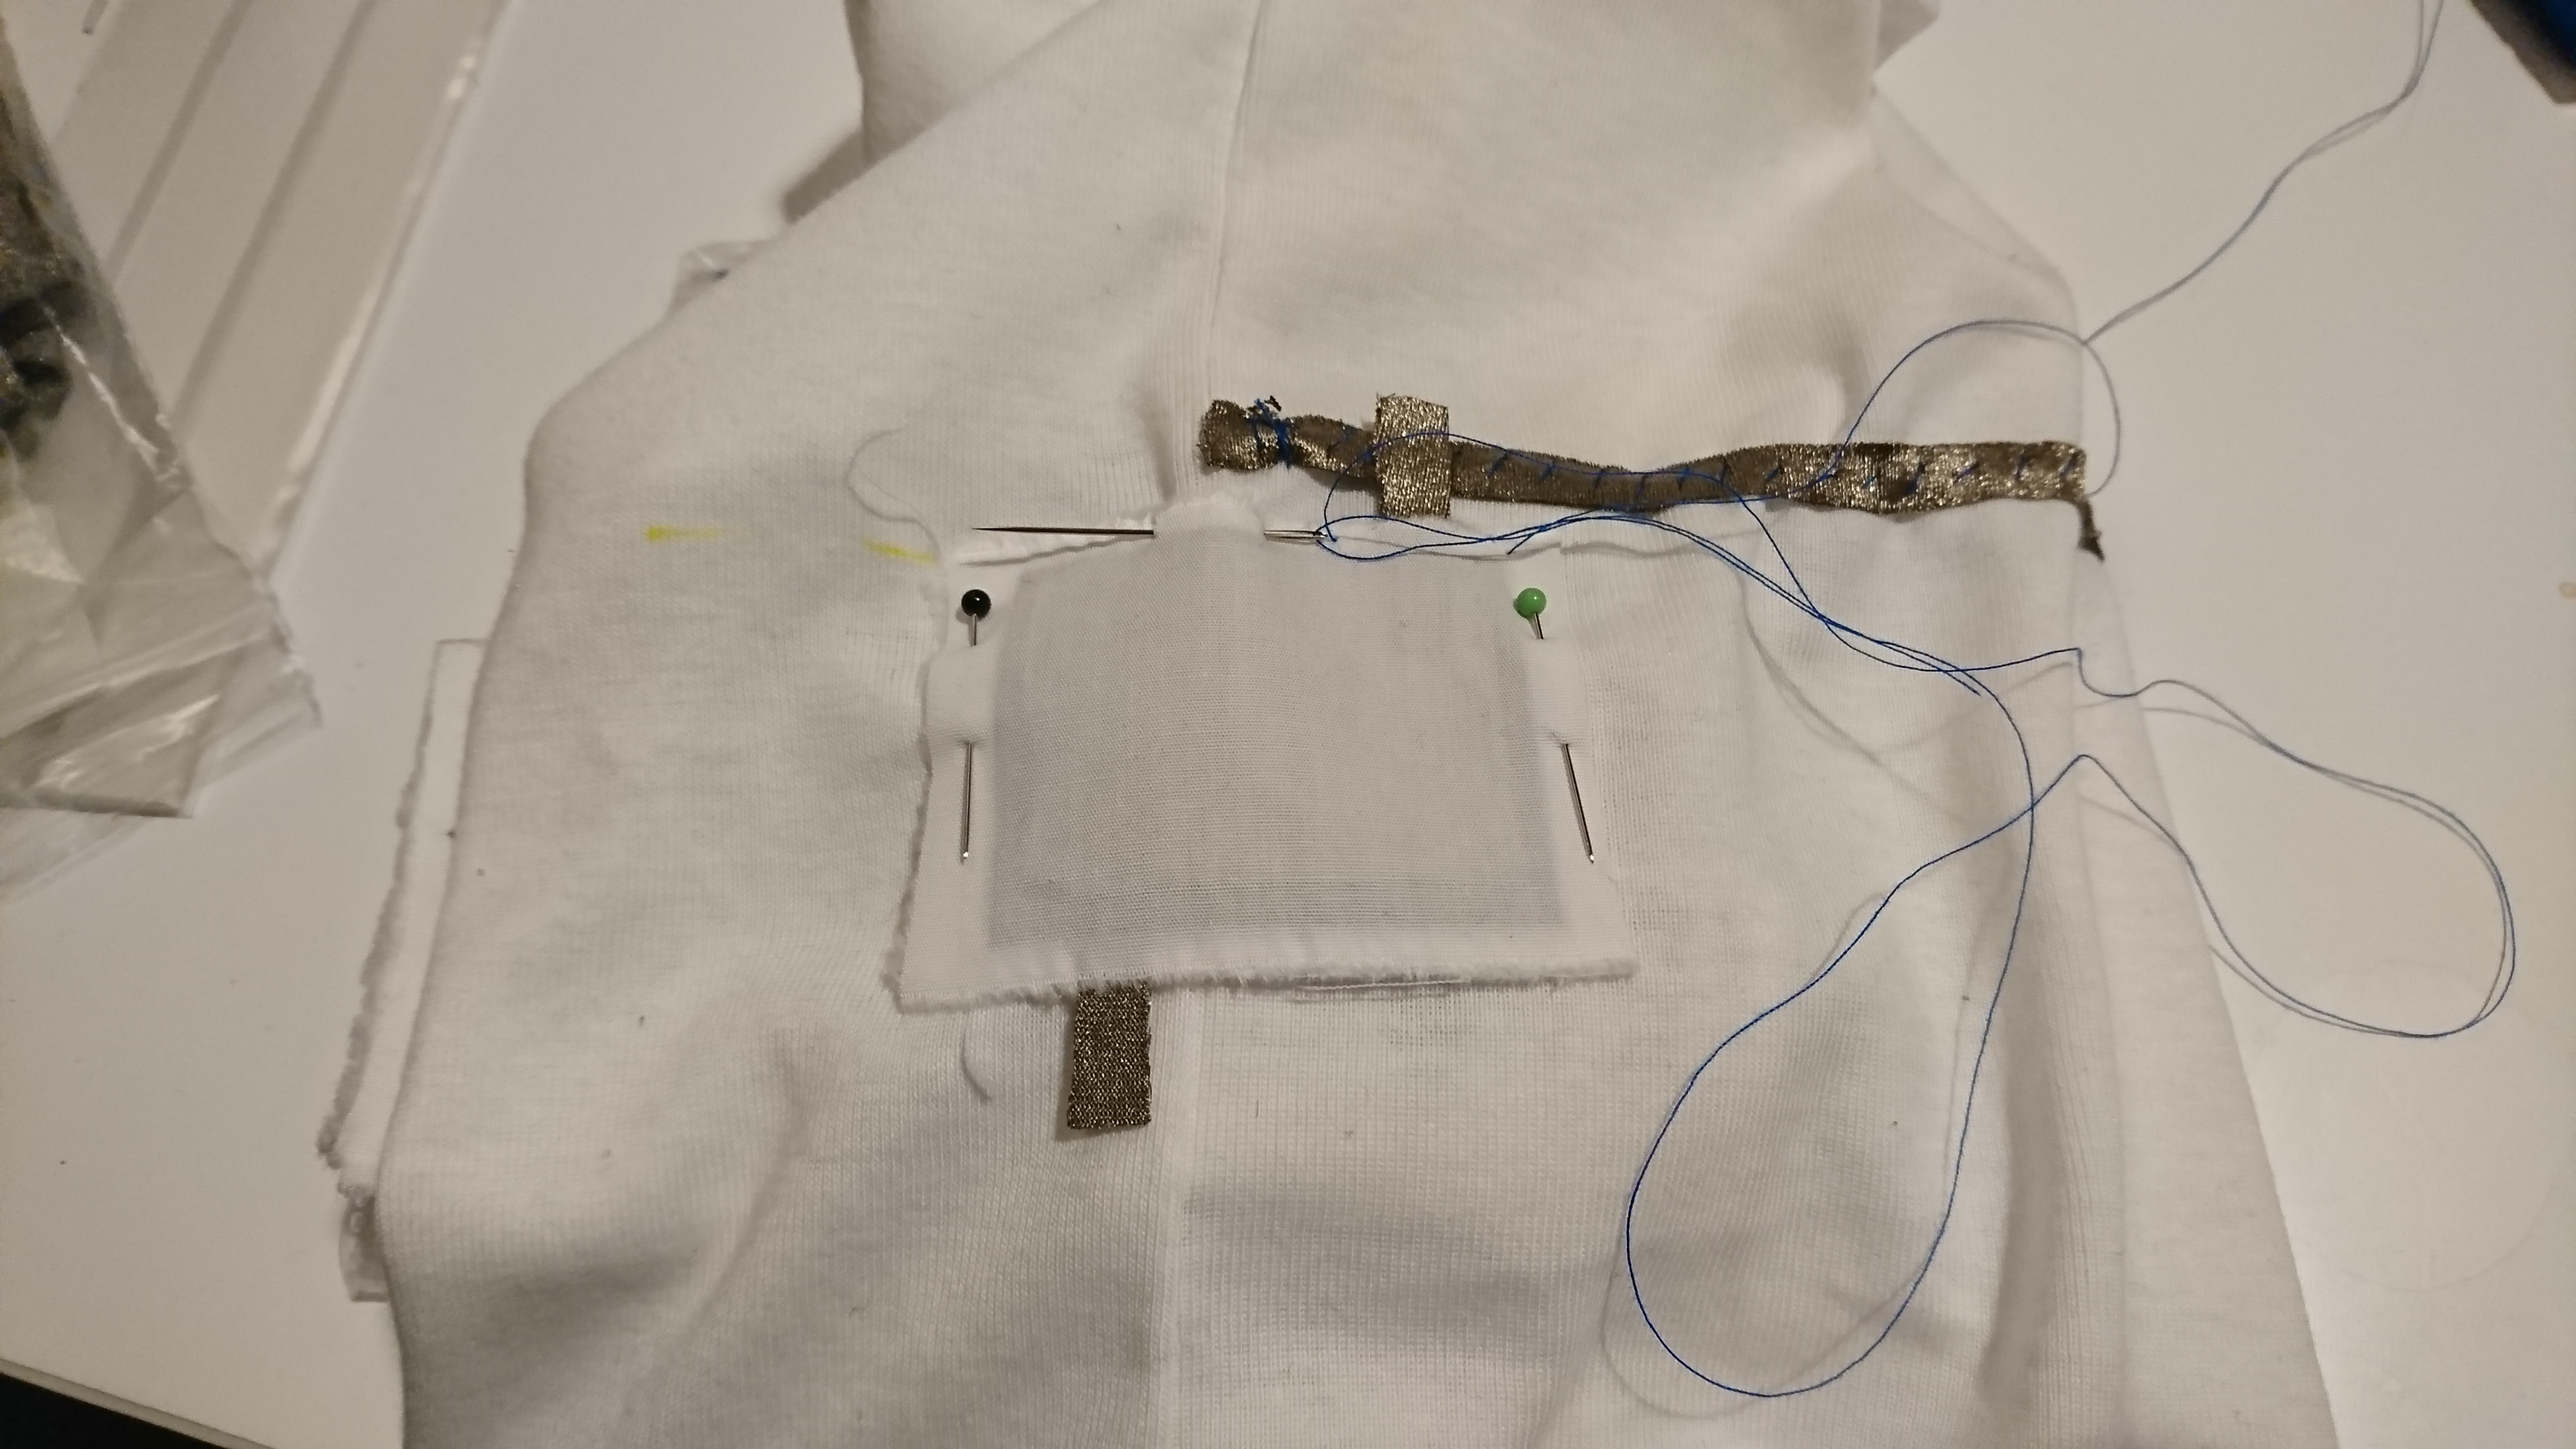
\includegraphics[width=0.85\textwidth]{img/pe_integration.JPG}
    \caption{Pressure sensor sewn into the onesie.}
\end{figure}
    \end{minipage}}\label{sec:sidebar3} } 
%\end{comment}
We cut a long strip of material which is 1 cm. wide, which we can test in various lengths.
Also, we have our original piece 5.4x9.5cm.

\begin{table}
  \centering
  \begin{tabular}{l r r r r}
    % \toprule
    & \multicolumn{4}{l}{\small{\textbf{Breath circumference measure}}} \\
    \cmidrule(r){1-2}
    {\small\textit{Size (cm x cm)}}
    & {\small \textit{0 cm}} 
    & {\small \textit{1 cm}} 
    & {\small \textit{2 cm}} 
    & {\small \textit{3 cm}} \\
    \midrule
    3x1    & 0.101 & 0.109 & 0.102 & - \\
    5x2    & 0.181 & 0.174 & 0.164 & 0.155 \\
    7x1    & 0.223 & 0.214 & 0.209 & 0.205 \\
    9x1    & 0.263 & 0.256 & 0.252 & 0.252 \\
    11x1    & 0.341 & 0.329 & 0.323 & 0.318 \\
    % \bottomrule
  \end{tabular}
  \caption{Resistance measured using volt-meter at 2M}~\label{tab:circumference}
\end{table}

\colorbox{cyan}{Measuring this way does not work as intended}.\\
\colorbox{cyan}{Need more stability when stretching the fabric...}.

\subsection{Pressure sensors}
The position sensors will be eTextile pressure sensors by putting two conductive
fabrics with a piezoresistive fabric in-between.\\
For testing
the efficiency of the sensor we started by making a 
simple prototype before the actual sensors.
We used some standard copper wires, 1.4 mm, after verifying the pad with
crocodile clip wires. When we tested this pad, the idle resistance measured when on the table was
900 or so. When touching it, it dropped to around 400. Even slight pressure
was detected.

After verifying that the pressure sensor can be used as 
intended. We manufactured with as much precision as possible
the actual sensors which will be used in the prototype. 

Instead of cobber wires, we will use silver plated nylon
with which has high conductivity. When tested we experienced
the same behaviour as when using cobber wiring.

As before all the conductive fabrics (non stretch) were 
burned around the edges to keep the fabric from fraying.
For wrapping and keeping in place, we used a thin cotton 
fabric which is non-conductive and kept together by
fabric glue.
For connectors we use the silver plated nylon fabric to make a stripe around
the stomach for the ground connector which all pads will be connected to.\\
For the wiring of each of the analog input to each pad, we used conductive thread
which uses the same silver plating to make it conductive.\\
We could also have used the fabric here. However, we would have to solve the problem
of insulating each strip, as the limited space on the onesie could result in overlapping
connectors.



\clearpage

\section{Software/setup}
\colorbox{cyan}{A little about how our Arduino-setup works with plots}.


\section{Prototype evaluation}
\colorbox{cyan}{How will this be done?}.

\section{Future work}
\colorbox{cyan}{Sensors work}.

\colorbox{cyan}{Breath sensor is viable theoretically?}.

\colorbox{cyan}{ACTUAL BABY?}.

\section{Conclusion}
\colorbox{cyan}{The paper is concluded}.




\balance{} 

\bibliographystyle{SIGCHI-Reference-Format}
\bibliography{sample}

\end{document}

%%% Local Variables:
%%% mode: latex
%%% TeX-master: t
%%% End:
